\section{Auswirkung der OLAP-Engine}\label{auswertung:olap}
Bei der Analyse von Query 1.2 ist aufgefallen, dass der Query manchmal über die OLAP-Engine 
ausgeführt\footnote{Um zu sehen, welche Engine verwendet wird, muss anstatt \enquote{Visualize Plan} die Option \enquote{Explain Plan} gewählt werden.} wird. 
Die OLAP-Engine ist speziell für \enquote{Analytical Views}, die als Columnstore im Star-Schema vorliegen, gedacht.\cite{olap,olap2} Beim Star-Schema Benchmark liegen die Daten definitv im Star-Schema vor.


%http://saphanatutorial.com/sap-hana-modeling/
%https://archive.sap.com/discussions/thread/3340726
Zunächst trat die OLAP-Engine nur auf, wenn Indizes hinzugefügt wurden, weshalb zunächst angenommen wurde, dass
 HANA an Hand der Indizes erkennt, dass es sich im Grunde um einen Analytical View handelt und dementsprechend optimiert.
Allerdings gab es auch Fälle, wo die OLAP-Engine auch ohne Indizes verwendet wurde. Warum die OLAP-Engine scheinbar zufällig verwendet wurde, ist unklar.

Soll gezielt die OLAP-Engine genutzt werden, so kann dies durch den Hint \enquote{USE\_OLAP\_PLAN} erzwungen werden.\cite{olap3,olap5}
Um die Auswirkung der OLAP-Engine genauer zu untersuchen, wurden die Benchmarks mit/ohne Indidzes, siehe \autoref{auswertung:basic_indizes}, jeweils mit und ohne den OLAP-Hint ausgeführt.


\begin{figure}[H]
    \centering
    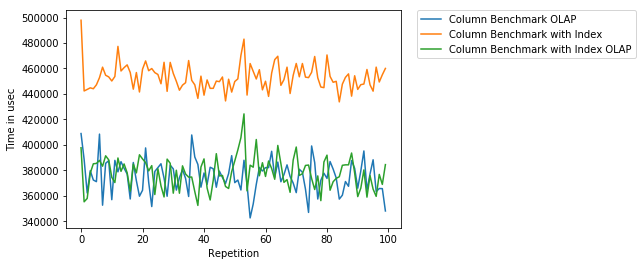
\includegraphics[width=0.49\textwidth]{olap_column_overall.png}
    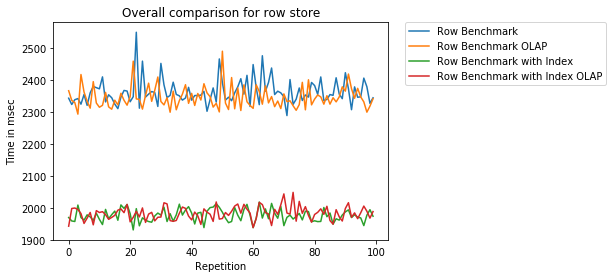
\includegraphics[width=0.49\textwidth]{olap_row_overall.png}
    \caption{Vergleich der Gesamtlaufzeit mit OLAP-Hint. n=100}
	\label{fig:olap_overall}
\end{figure}

\subsection{Untersuchung für Columnstore}
Beim Vergleich der verschiedenen Kombinationen für Columstores war das Ergebnis eindeutig: Die OLAP-Engine schlägt die normale Column-Engine um Längen.

Im Schnitt ist die OLAP-Engine 38 ms schneller, als die Column-Engine mit Indizes. Lässt man die Indizes weg wird der Unterschied noch größer, da die Column-Engine langsamer wird.
 Die OLAP-Engine scheint von den Inidzes nicht beeinflusst zu werden, siehe \autoref{tab:olap}.

%https://www.stechies.com/important-hints-related-sap-hana/
\setlength\intextsep{0pt}
\begin{wraptable}{r}{0.5\textwidth}
    \begin{tabular}{ccc}
        \toprule
        Engine              & No Index [ms]   & Index [ms] \\
        \toprule
        OLAP                & 187        & 188            \\
        Colum               & 296        & 226            \\   
        \bottomrule
    \end{tabular}
	\caption{Durchschnitt der Gesamtlaufzeit mit und ohne OLAP-Engine bei Columnstore.}
    \label{tab:olap}
\end{wraptable}

Bei genauerer Betrachtung der Laufzeit pro Benchmarkgruppe fällt besonders auf, dass die Querys der Gruppe 1 nicht von der OLAP-Engine profitieren, sondern sogar langsamer werden. 

Die anderen Benchmarkgruppen werden durch den OLAP-Hint jedoch schneller, Gruppe 3 und 4 nur geringfügig, Gruppe 2 jedoch wird nahezu doppelt so schnell.
\begin{table}[H]
    \centering
    \begin{tabularx}{\textwidth}{lXrrrr}
    \toprule
	Wert        &	OLAP-Hint & Q1 	    &	Q2 	    &	Q3	    &	Q4 \\
    \toprule
    Average	    & Nein        &	23.5	&	72.5	&	60.4	&	69.9 \\
    Average     & Ja	      &	26.3	&	36.4	&	58.3	&	65.6 \\
    \midrule
    Median	    & Nein        &	23.4	&	72.1	&	60.2	&	69.3 \\
    Median	    & Ja          &	26.5	&	36.0	&	59.5	&	66.0 \\
    \bottomrule
    \end{tabularx}
	\caption{Laufzeit jeder Benchmarkgruppe für Columnstore mit Index, testweise mit OLAP-Hint. n=100}
    \label{tab:olap_bench}
\end{table}
%Hier dann Tabelle, wenn Benchmark fertig ist. 
\setlength\intextsep{0pt}
\subsection{Untersuchungen für Rowstore}
\begin{wraptable}{r}{0.5\textwidth}
    \begin{tabular}{ccc}
        \toprule
        Engine              & No Index [ms]   & Index [ms] \\
        \toprule
        OLAP                & 2362        & 1976           \\
        Row                 & 2344        & 1977           \\   
        \bottomrule
    \end{tabular}
	\caption{Durchschnitt der Gesamtlaufzeit mit und ohne OLAP-Engine bei Rowstore.}
    \label{tab:olap}
\end{wraptable}

Bei der Untersuchung der Ergebnisse für Rowstore und wie bereits in \autoref{fig:olap_overall} zu sehen, hat die OLAP-Engine keine Auswirkung auf die Laufzeit des Benchmarks.

Vermutlich liegt dies daran, dass die OLAP-Engine nur auf Analytical-Views, die im Columnstore gespeichert sind, ausgelegt ist. Überprüft wurde dies aber nicht.



\subsection{Fazit}
Durch Nutzung der OLAP-Engine kann man eventuelle Beschleunigungen durch Indizes, zumindest für Columnstores, nochmals deutlich überbieten.
Es erscheint sinnvoller, sein Augenmerk darauf zu legen, dass Querys diese auch nutzen. Dies ist zwar über einen HINT möglich, davon wird in der Praxis jedoch abgeraten.\cite{olap4}
Alternativ könnte man seine Anfragen \enquote{formgerecht} als Analytical-View aufbauen, um die OLAP-Engine nutzen zu können.\cite{olap6,olap2}

Für Rowstores kann die OLAP-Engine leider nicht verwendet werden.
%https://archive.sap.com/discussions/thread/3277920
